\documentclass[11pt]{article}
\usepackage[textwidth=18.0cm, textheight=23.0cm, top=2.0cm]{geometry}
\usepackage{pst-all}
\usepackage{amssymb}
\usepackage{tikz}
\usepackage{underscore}\begin{document}
\pagestyle{empty}


ClassName: \underline{\textbf{Class_10.2bp-10}}
\par
BinSize: \underline{\textbf{100 × 100}}
\par
ReduceSize: \underline{\textbf{100 × 100}}
\par
TypeNum: \underline{\textbf{40}}
\par
Num: \underline{\textbf{40}}
\par
OutS: \underline{\textbf{80000}}
\par
InS: \underline{\textbf{70283}}
\par
Rate: \underline{\textbf{0.879}}
\par
UB: \underline{\textbf{8}}
\par
LB0: \underline{\textbf{8}}
\par
LB: \underline{\textbf{8}}
\par
LBWithCut: \underline{\textbf{8}}
\par
NodeCut: \underline{\textbf{0}}
\par
ExtendedNodeCnt: \underline{\textbf{1}}
\par
GenNodeCnt: \underline{\textbf{1}}
\par
PrimalNode: \underline{\textbf{0}}
\par
ColumnCount: \underline{\textbf{8}}
\par
TotalCutCount: \underline{\textbf{0}}
\par
RootCutCount: \underline{\textbf{0}}
\par
LPSolverCnt: \underline{\textbf{1}}
\par
PricingSolverCnt: \underline{\textbf{0}}
\par
BranchAndBoundNum: \underline{\textbf{1}}
\par
isOpt: \underline{\textbf{true}}
\par
TimeOnInitSolution: \underline{\textbf{600.000 s}}
\par
TimeOnPrimal: \underline{\textbf{0.000 s}}
\par
TimeOnPricing: \underline{\textbf{0.000 s}}
\par
TimeOnRmp: \underline{\textbf{0.070 s}}
\par
TotalTime: \underline{\textbf{600.332 s}}
\par
\newpage


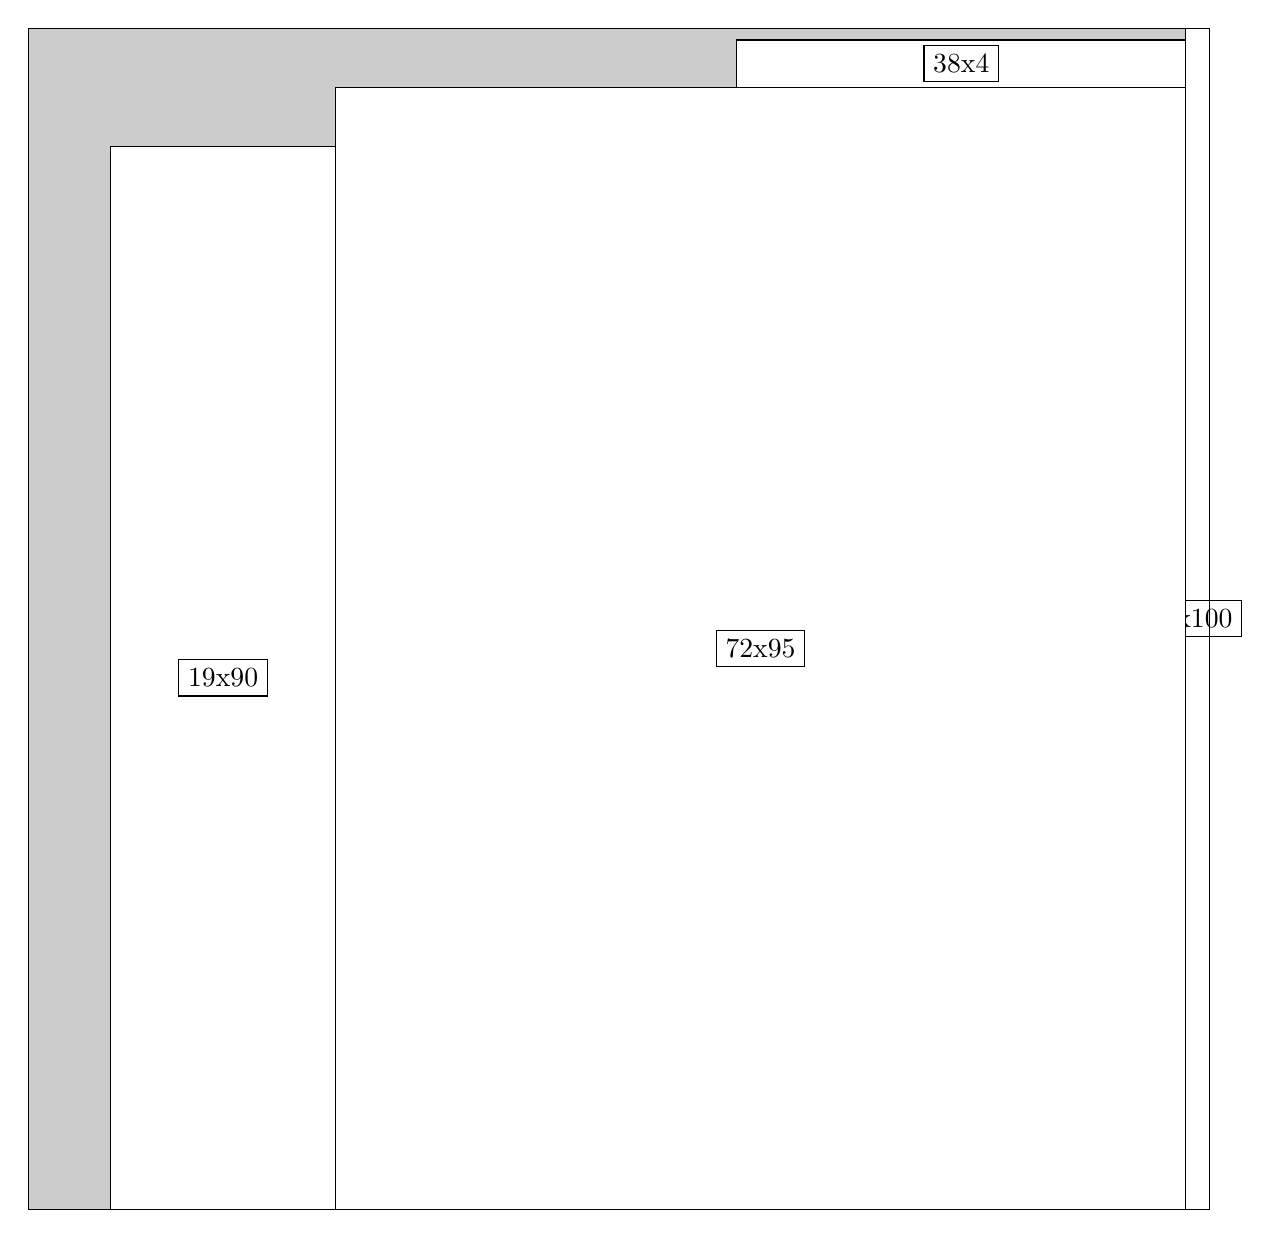
\begin{tikzpicture}[shorten >=1pt,scale=1.0,every node/.style={scale=1.0},->]
\tikzstyle{vertex}=[circle,fill=black!25,minimum size=14pt,inner sep=0pt]
\filldraw[fill=gray!40!white, draw=black] (0,0) rectangle (15.0,15.0);
\foreach \name/\x/\y/\w/\h in {2x100/14.7/0.0/0.3/15.0,72x95/3.9/0.0/10.799999999999999/14.25,38x4/9.0/14.25/5.7/0.6,19x90/1.05/0.0/2.85/13.5}
\filldraw[fill=white!40!white, draw=black] (\x,\y) rectangle node[draw] (\name) {\name} ++(\w,\h);
\end{tikzpicture}


w =2 , h =100 , x =98 , y =0 , v =200
\par
w =72 , h =95 , x =26 , y =0 , v =6840
\par
w =38 , h =4 , x =60 , y =95 , v =152
\par
w =19 , h =90 , x =7 , y =0 , v =1710
\par
\newpage


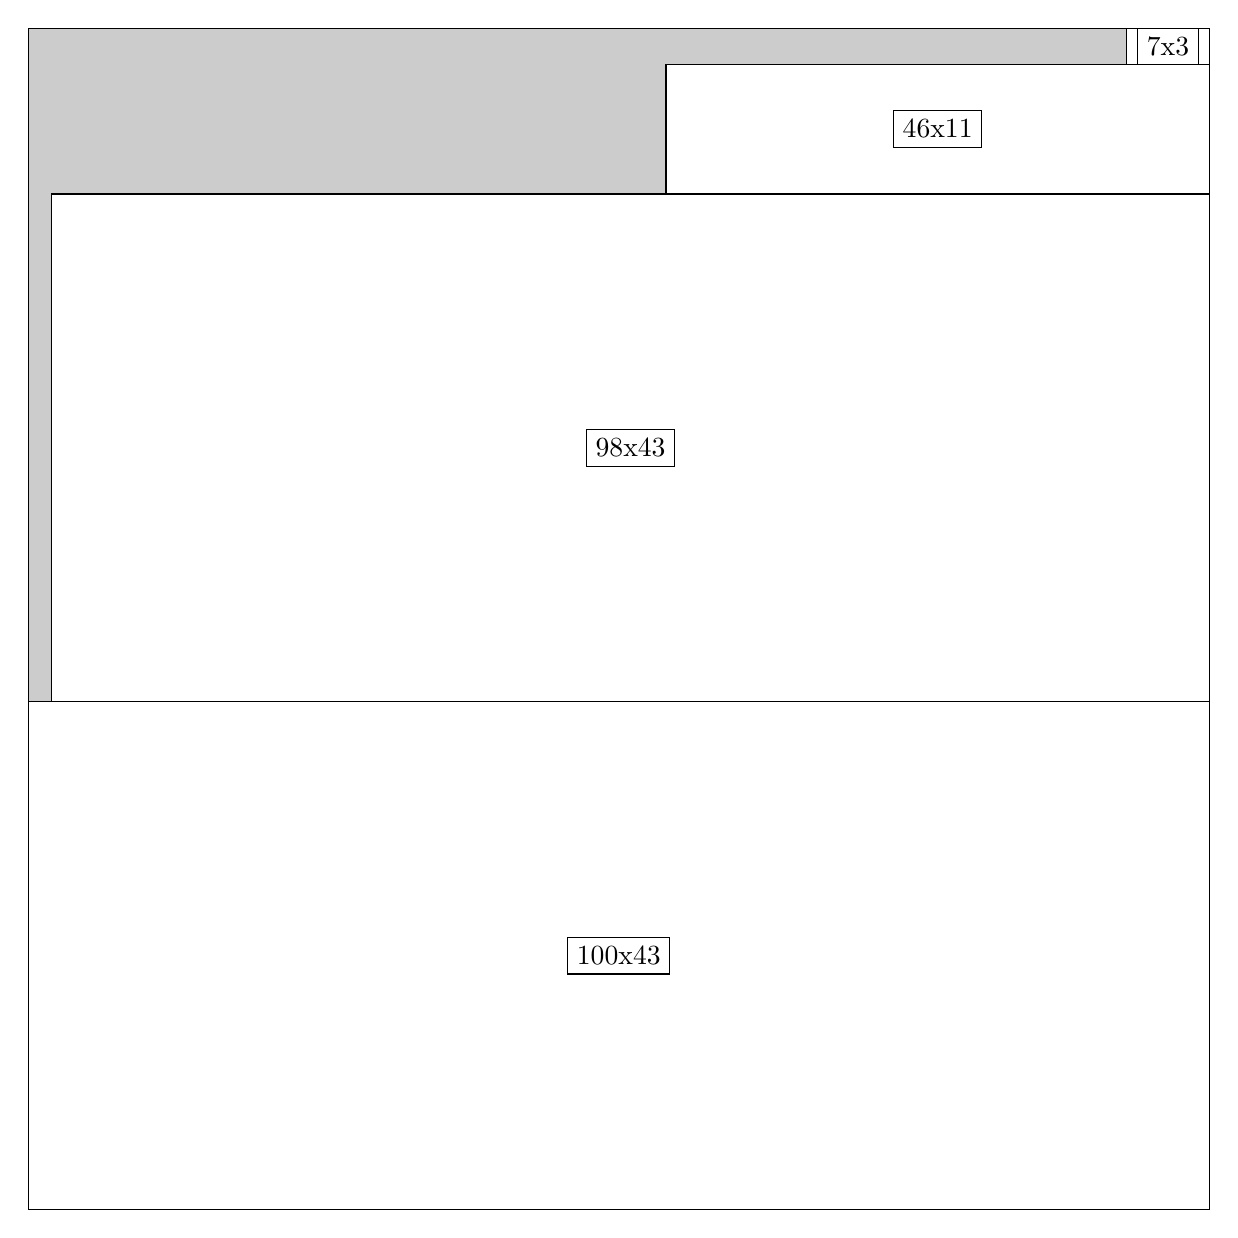
\begin{tikzpicture}[shorten >=1pt,scale=1.0,every node/.style={scale=1.0},->]
\tikzstyle{vertex}=[circle,fill=black!25,minimum size=14pt,inner sep=0pt]
\filldraw[fill=gray!40!white, draw=black] (0,0) rectangle (15.0,15.0);
\foreach \name/\x/\y/\w/\h in {100x43/0.0/0.0/15.0/6.45,98x43/0.3/6.45/14.7/6.45,46x11/8.1/12.9/6.8999999999999995/1.65,7x3/13.95/14.549999999999999/1.05/0.44999999999999996}
\filldraw[fill=white!40!white, draw=black] (\x,\y) rectangle node[draw] (\name) {\name} ++(\w,\h);
\end{tikzpicture}


w =100 , h =43 , x =0 , y =0 , v =4300
\par
w =98 , h =43 , x =2 , y =43 , v =4214
\par
w =46 , h =11 , x =54 , y =86 , v =506
\par
w =7 , h =3 , x =93 , y =97 , v =21
\par
\newpage


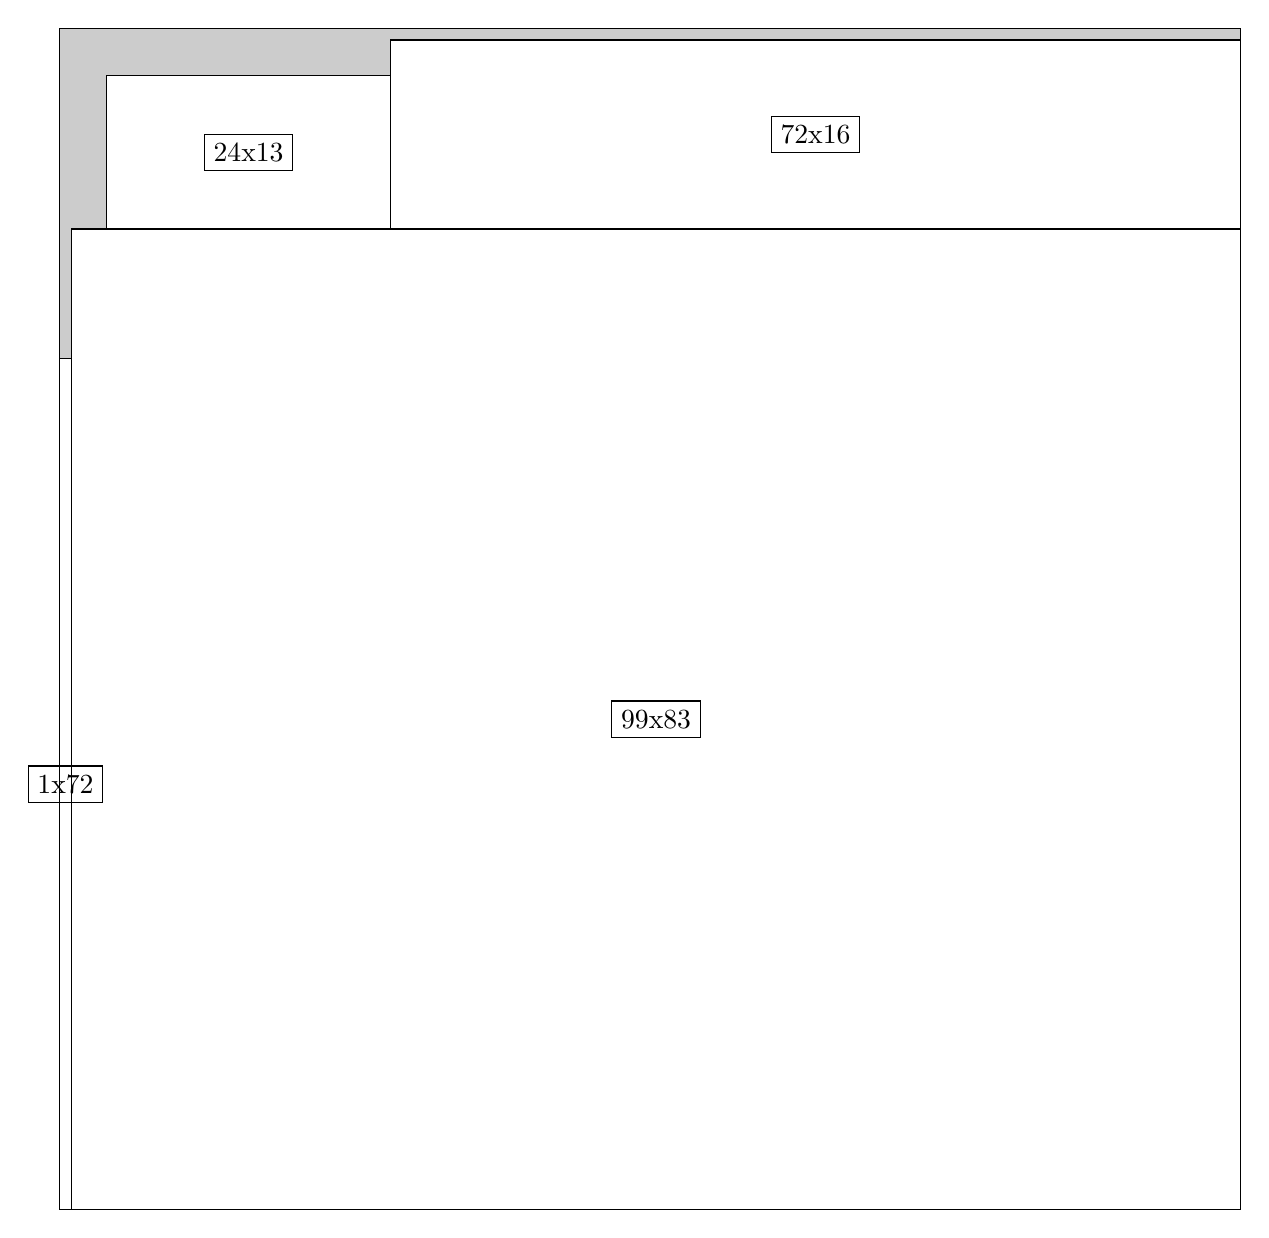
\begin{tikzpicture}[shorten >=1pt,scale=1.0,every node/.style={scale=1.0},->]
\tikzstyle{vertex}=[circle,fill=black!25,minimum size=14pt,inner sep=0pt]
\filldraw[fill=gray!40!white, draw=black] (0,0) rectangle (15.0,15.0);
\foreach \name/\x/\y/\w/\h in {99x83/0.15/0.0/14.85/12.45,1x72/0.0/0.0/0.15/10.799999999999999,72x16/4.2/12.45/10.799999999999999/2.4,24x13/0.6/12.45/3.5999999999999996/1.95}
\filldraw[fill=white!40!white, draw=black] (\x,\y) rectangle node[draw] (\name) {\name} ++(\w,\h);
\end{tikzpicture}


w =99 , h =83 , x =1 , y =0 , v =8217
\par
w =1 , h =72 , x =0 , y =0 , v =72
\par
w =72 , h =16 , x =28 , y =83 , v =1152
\par
w =24 , h =13 , x =4 , y =83 , v =312
\par
\newpage


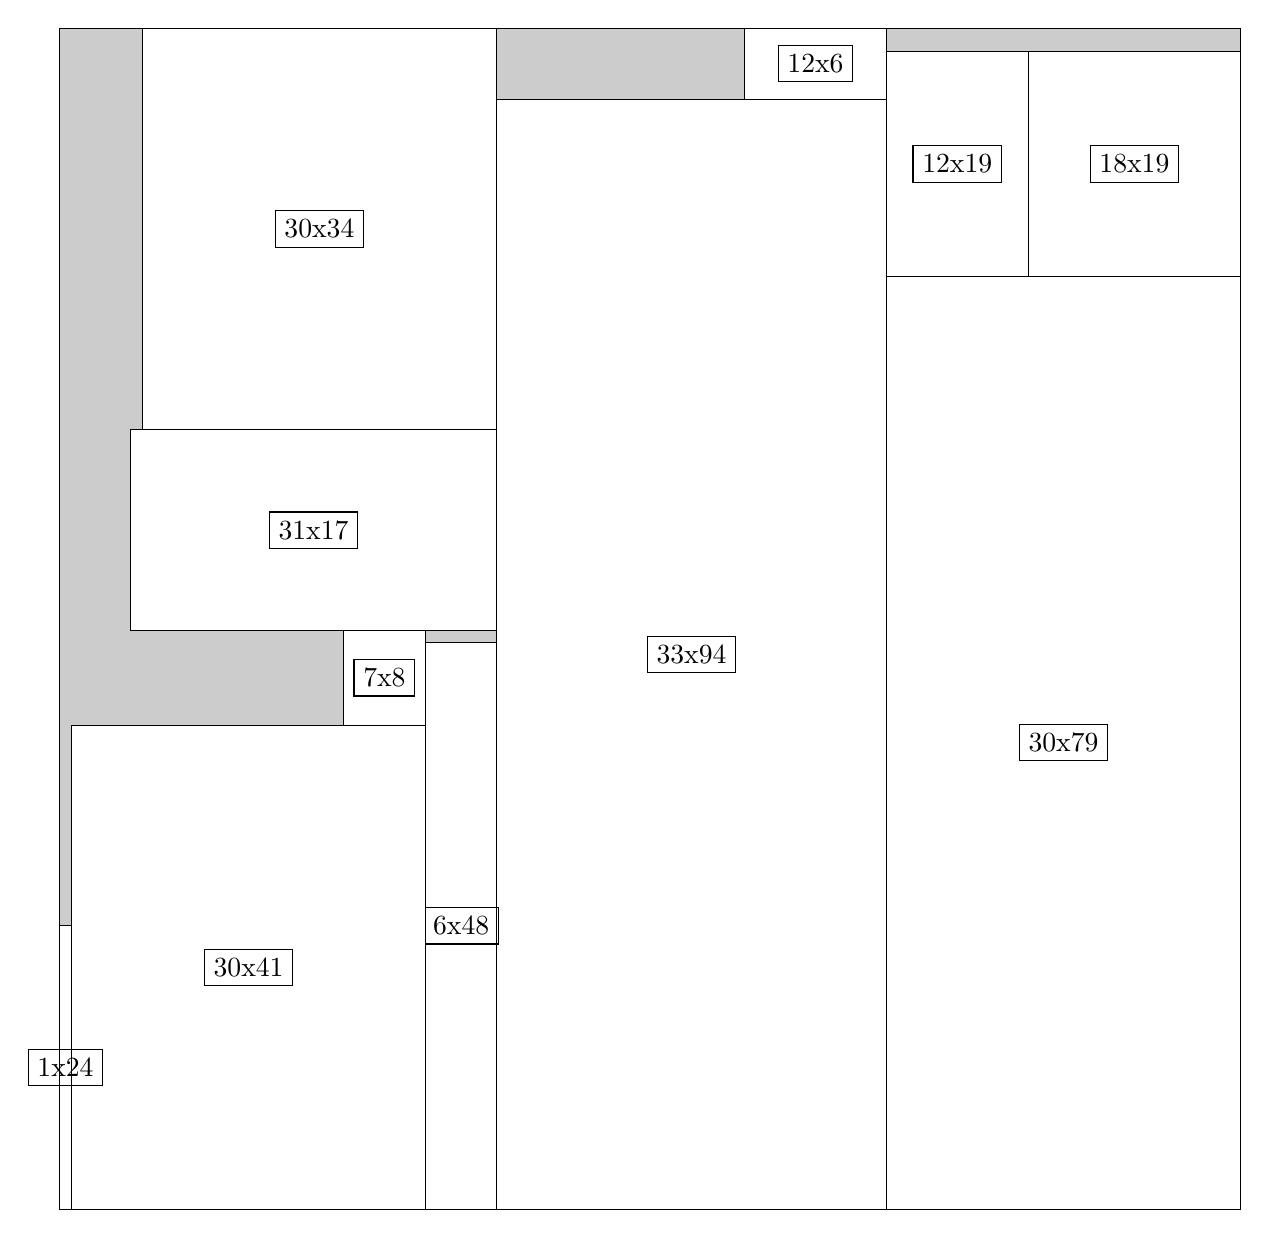
\begin{tikzpicture}[shorten >=1pt,scale=1.0,every node/.style={scale=1.0},->]
\tikzstyle{vertex}=[circle,fill=black!25,minimum size=14pt,inner sep=0pt]
\filldraw[fill=gray!40!white, draw=black] (0,0) rectangle (15.0,15.0);
\foreach \name/\x/\y/\w/\h in {30x79/10.5/0.0/4.5/11.85,18x19/12.299999999999999/11.85/2.6999999999999997/2.85,12x19/10.5/11.85/1.7999999999999998/2.85,33x94/5.55/0.0/4.95/14.1,12x6/8.7/14.1/1.7999999999999998/0.8999999999999999,6x48/4.6499999999999995/0.0/0.8999999999999999/7.199999999999999,30x41/0.15/0.0/4.5/6.1499999999999995,7x8/3.5999999999999996/6.1499999999999995/1.05/1.2,1x24/0.0/0.0/0.15/3.5999999999999996,31x17/0.8999999999999999/7.35/4.6499999999999995/2.55,30x34/1.05/9.9/4.5/5.1}
\filldraw[fill=white!40!white, draw=black] (\x,\y) rectangle node[draw] (\name) {\name} ++(\w,\h);
\end{tikzpicture}


w =30 , h =79 , x =70 , y =0 , v =2370
\par
w =18 , h =19 , x =82 , y =79 , v =342
\par
w =12 , h =19 , x =70 , y =79 , v =228
\par
w =33 , h =94 , x =37 , y =0 , v =3102
\par
w =12 , h =6 , x =58 , y =94 , v =72
\par
w =6 , h =48 , x =31 , y =0 , v =288
\par
w =30 , h =41 , x =1 , y =0 , v =1230
\par
w =7 , h =8 , x =24 , y =41 , v =56
\par
w =1 , h =24 , x =0 , y =0 , v =24
\par
w =31 , h =17 , x =6 , y =49 , v =527
\par
w =30 , h =34 , x =7 , y =66 , v =1020
\par
\newpage


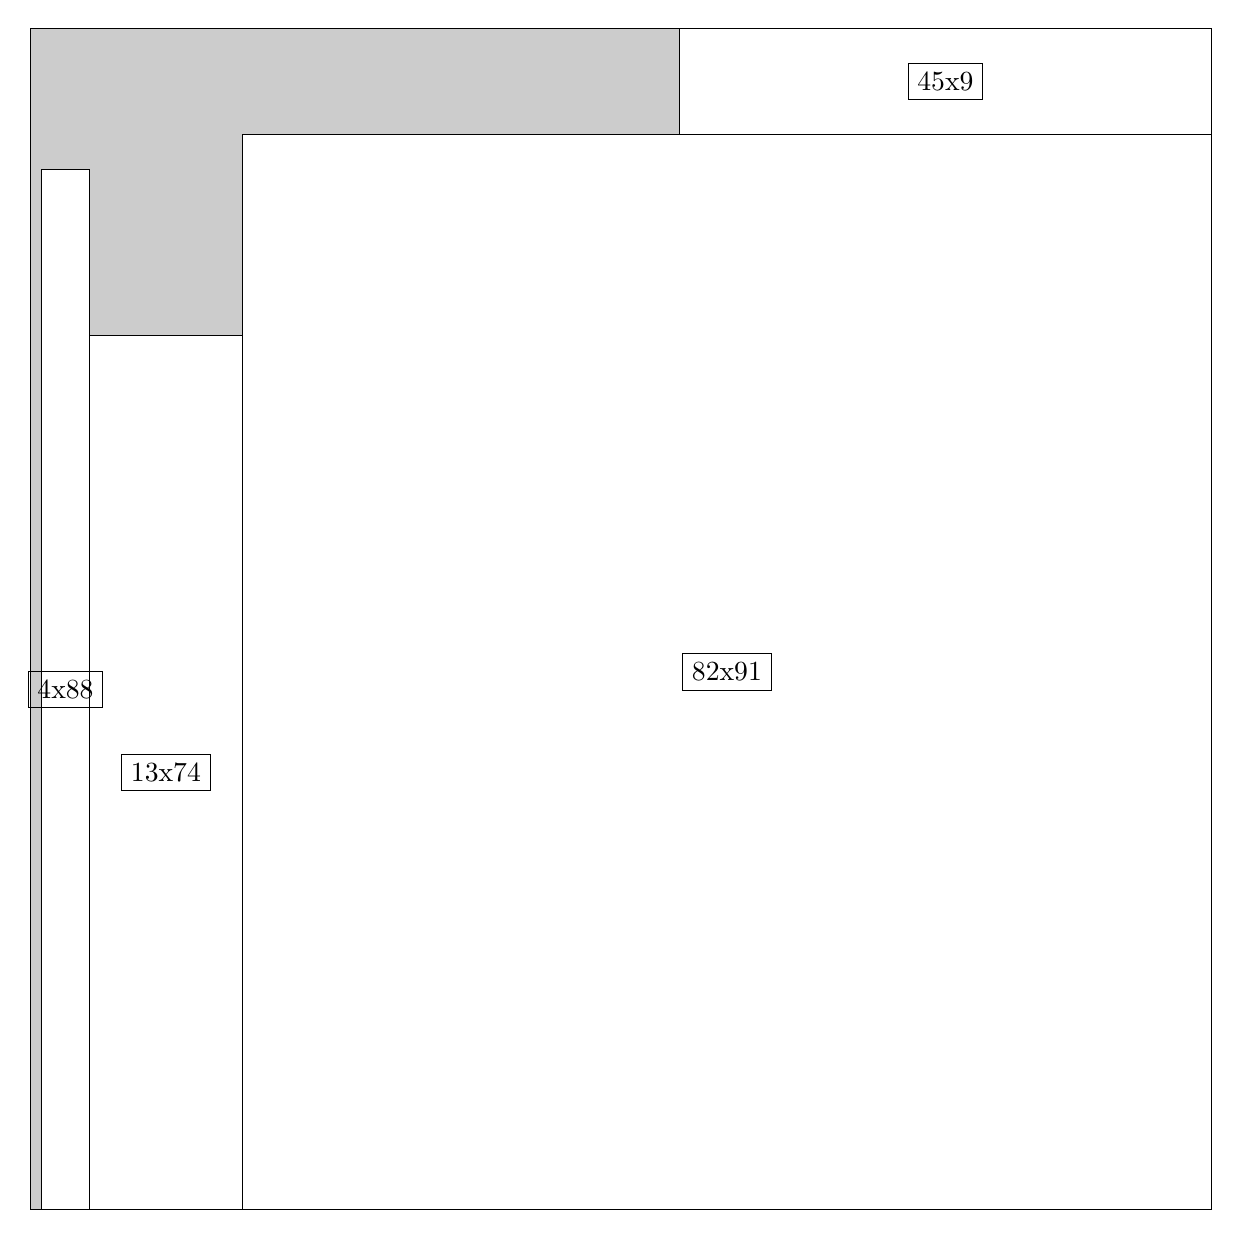
\begin{tikzpicture}[shorten >=1pt,scale=1.0,every node/.style={scale=1.0},->]
\tikzstyle{vertex}=[circle,fill=black!25,minimum size=14pt,inner sep=0pt]
\filldraw[fill=gray!40!white, draw=black] (0,0) rectangle (15.0,15.0);
\foreach \name/\x/\y/\w/\h in {82x91/2.6999999999999997/0.0/12.299999999999999/13.65,13x74/0.75/0.0/1.95/11.1,4x88/0.15/0.0/0.6/13.2,45x9/8.25/13.65/6.75/1.3499999999999999}
\filldraw[fill=white!40!white, draw=black] (\x,\y) rectangle node[draw] (\name) {\name} ++(\w,\h);
\end{tikzpicture}


w =82 , h =91 , x =18 , y =0 , v =7462
\par
w =13 , h =74 , x =5 , y =0 , v =962
\par
w =4 , h =88 , x =1 , y =0 , v =352
\par
w =45 , h =9 , x =55 , y =91 , v =405
\par
\newpage


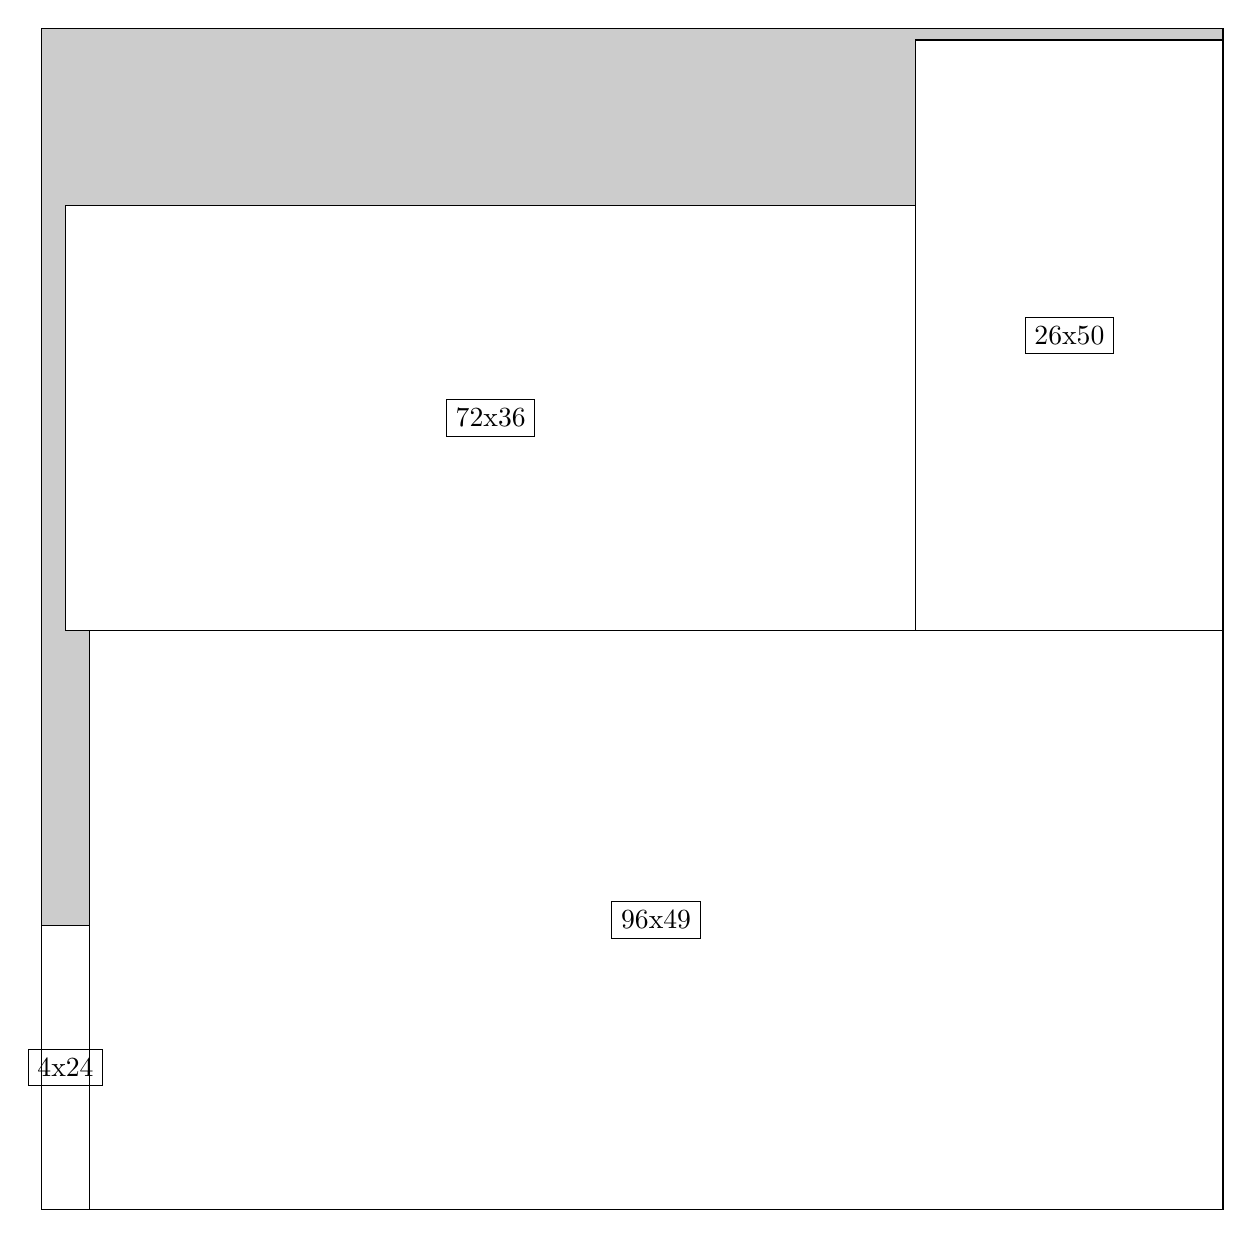
\begin{tikzpicture}[shorten >=1pt,scale=1.0,every node/.style={scale=1.0},->]
\tikzstyle{vertex}=[circle,fill=black!25,minimum size=14pt,inner sep=0pt]
\filldraw[fill=gray!40!white, draw=black] (0,0) rectangle (15.0,15.0);
\foreach \name/\x/\y/\w/\h in {96x49/0.6/0.0/14.399999999999999/7.35,4x24/0.0/0.0/0.6/3.5999999999999996,26x50/11.1/7.35/3.9/7.5,72x36/0.3/7.35/10.799999999999999/5.3999999999999995}
\filldraw[fill=white!40!white, draw=black] (\x,\y) rectangle node[draw] (\name) {\name} ++(\w,\h);
\end{tikzpicture}


w =96 , h =49 , x =4 , y =0 , v =4704
\par
w =4 , h =24 , x =0 , y =0 , v =96
\par
w =26 , h =50 , x =74 , y =49 , v =1300
\par
w =72 , h =36 , x =2 , y =49 , v =2592
\par
\newpage


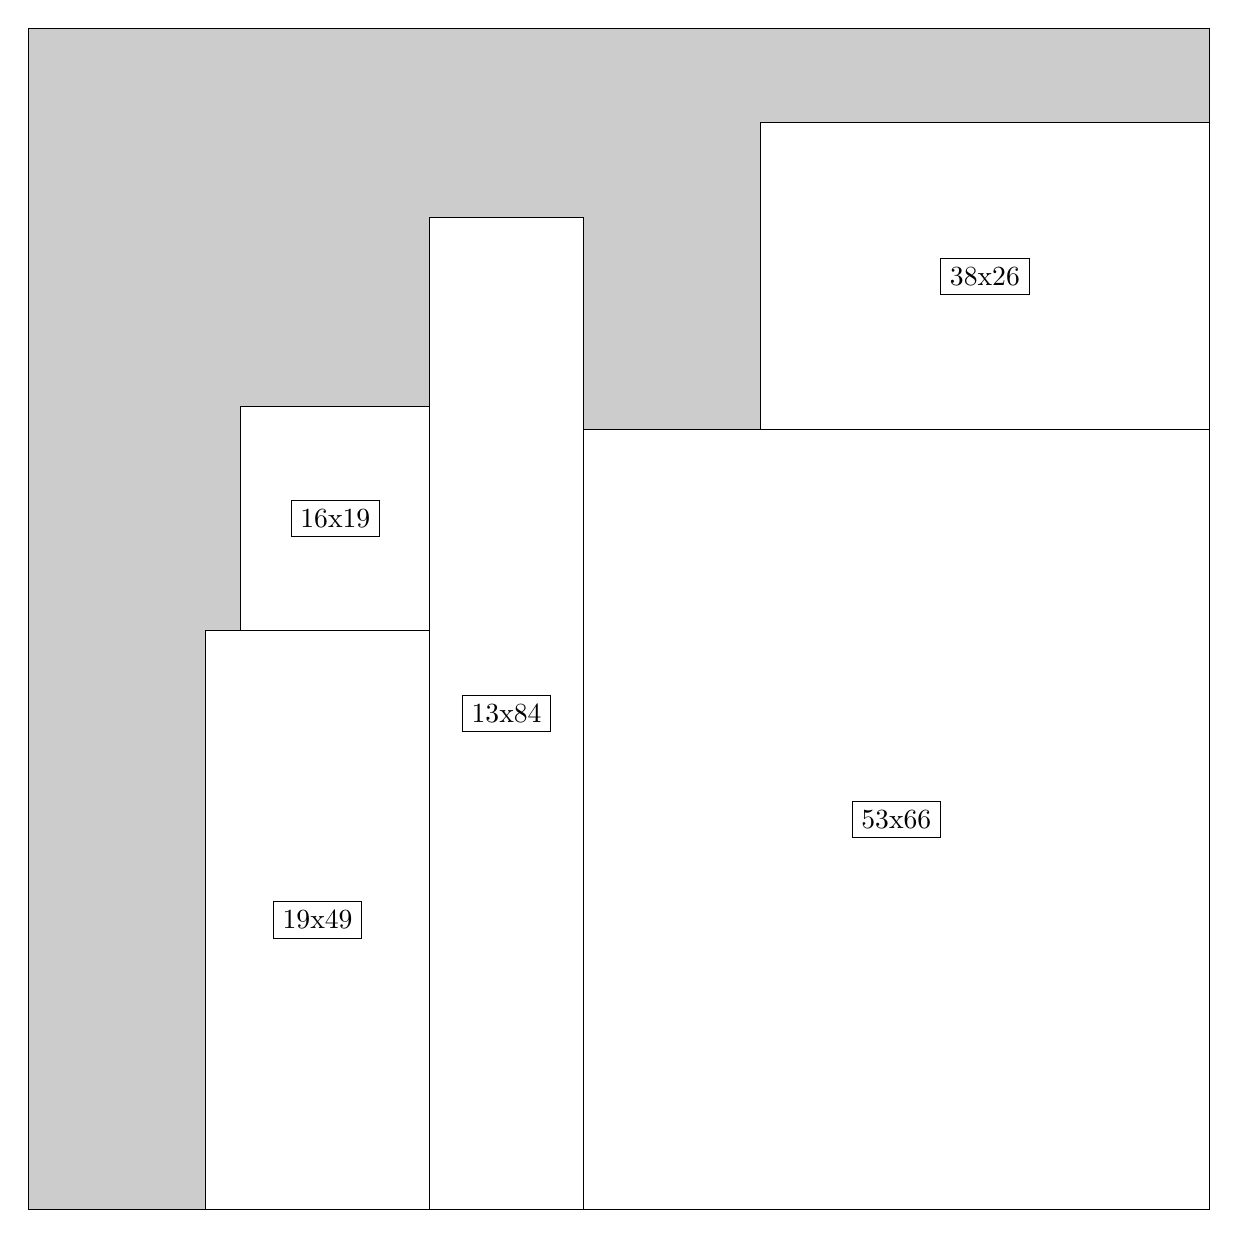
\begin{tikzpicture}[shorten >=1pt,scale=1.0,every node/.style={scale=1.0},->]
\tikzstyle{vertex}=[circle,fill=black!25,minimum size=14pt,inner sep=0pt]
\filldraw[fill=gray!40!white, draw=black] (0,0) rectangle (15.0,15.0);
\foreach \name/\x/\y/\w/\h in {53x66/7.05/0.0/7.949999999999999/9.9,38x26/9.299999999999999/9.9/5.7/3.9,13x84/5.1/0.0/1.95/12.6,19x49/2.25/0.0/2.85/7.35,16x19/2.6999999999999997/7.35/2.4/2.85}
\filldraw[fill=white!40!white, draw=black] (\x,\y) rectangle node[draw] (\name) {\name} ++(\w,\h);
\end{tikzpicture}


w =53 , h =66 , x =47 , y =0 , v =3498
\par
w =38 , h =26 , x =62 , y =66 , v =988
\par
w =13 , h =84 , x =34 , y =0 , v =1092
\par
w =19 , h =49 , x =15 , y =0 , v =931
\par
w =16 , h =19 , x =18 , y =49 , v =304
\par
\newpage


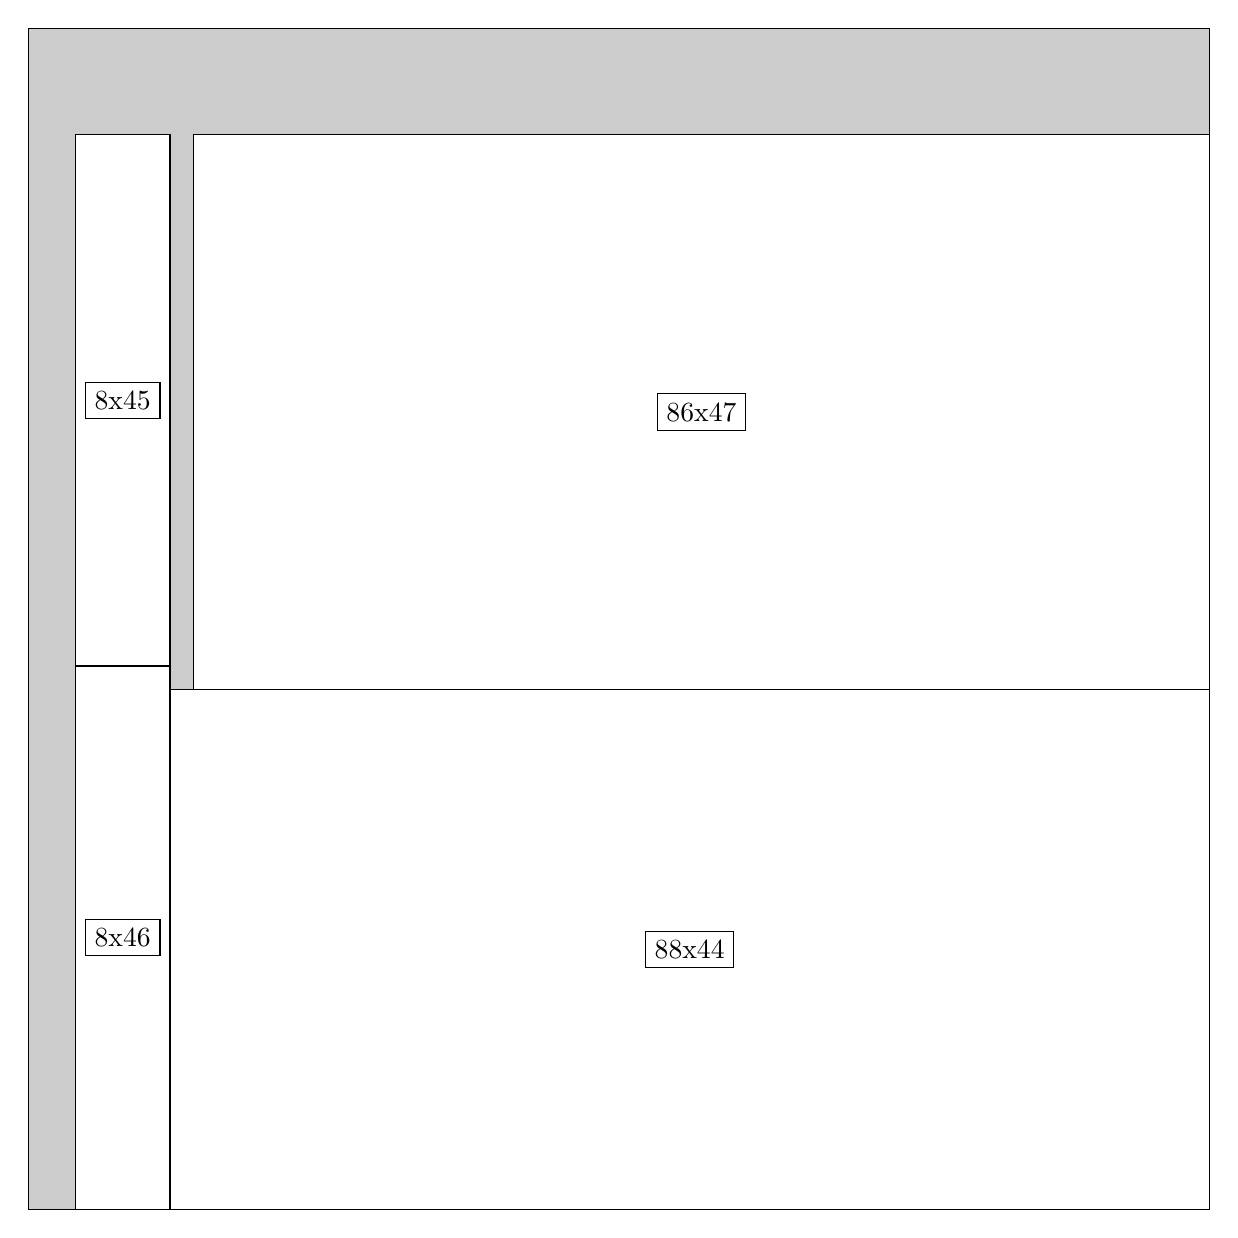
\begin{tikzpicture}[shorten >=1pt,scale=1.0,every node/.style={scale=1.0},->]
\tikzstyle{vertex}=[circle,fill=black!25,minimum size=14pt,inner sep=0pt]
\filldraw[fill=gray!40!white, draw=black] (0,0) rectangle (15.0,15.0);
\foreach \name/\x/\y/\w/\h in {88x44/1.7999999999999998/0.0/13.2/6.6,86x47/2.1/6.6/12.9/7.05,8x46/0.6/0.0/1.2/6.8999999999999995,8x45/0.6/6.8999999999999995/1.2/6.75}
\filldraw[fill=white!40!white, draw=black] (\x,\y) rectangle node[draw] (\name) {\name} ++(\w,\h);
\end{tikzpicture}


w =88 , h =44 , x =12 , y =0 , v =3872
\par
w =86 , h =47 , x =14 , y =44 , v =4042
\par
w =8 , h =46 , x =4 , y =0 , v =368
\par
w =8 , h =45 , x =4 , y =46 , v =360
\par
\newpage


\end{document}